
\section{Appendix}


\begin{figure*}[htb!]
\centering
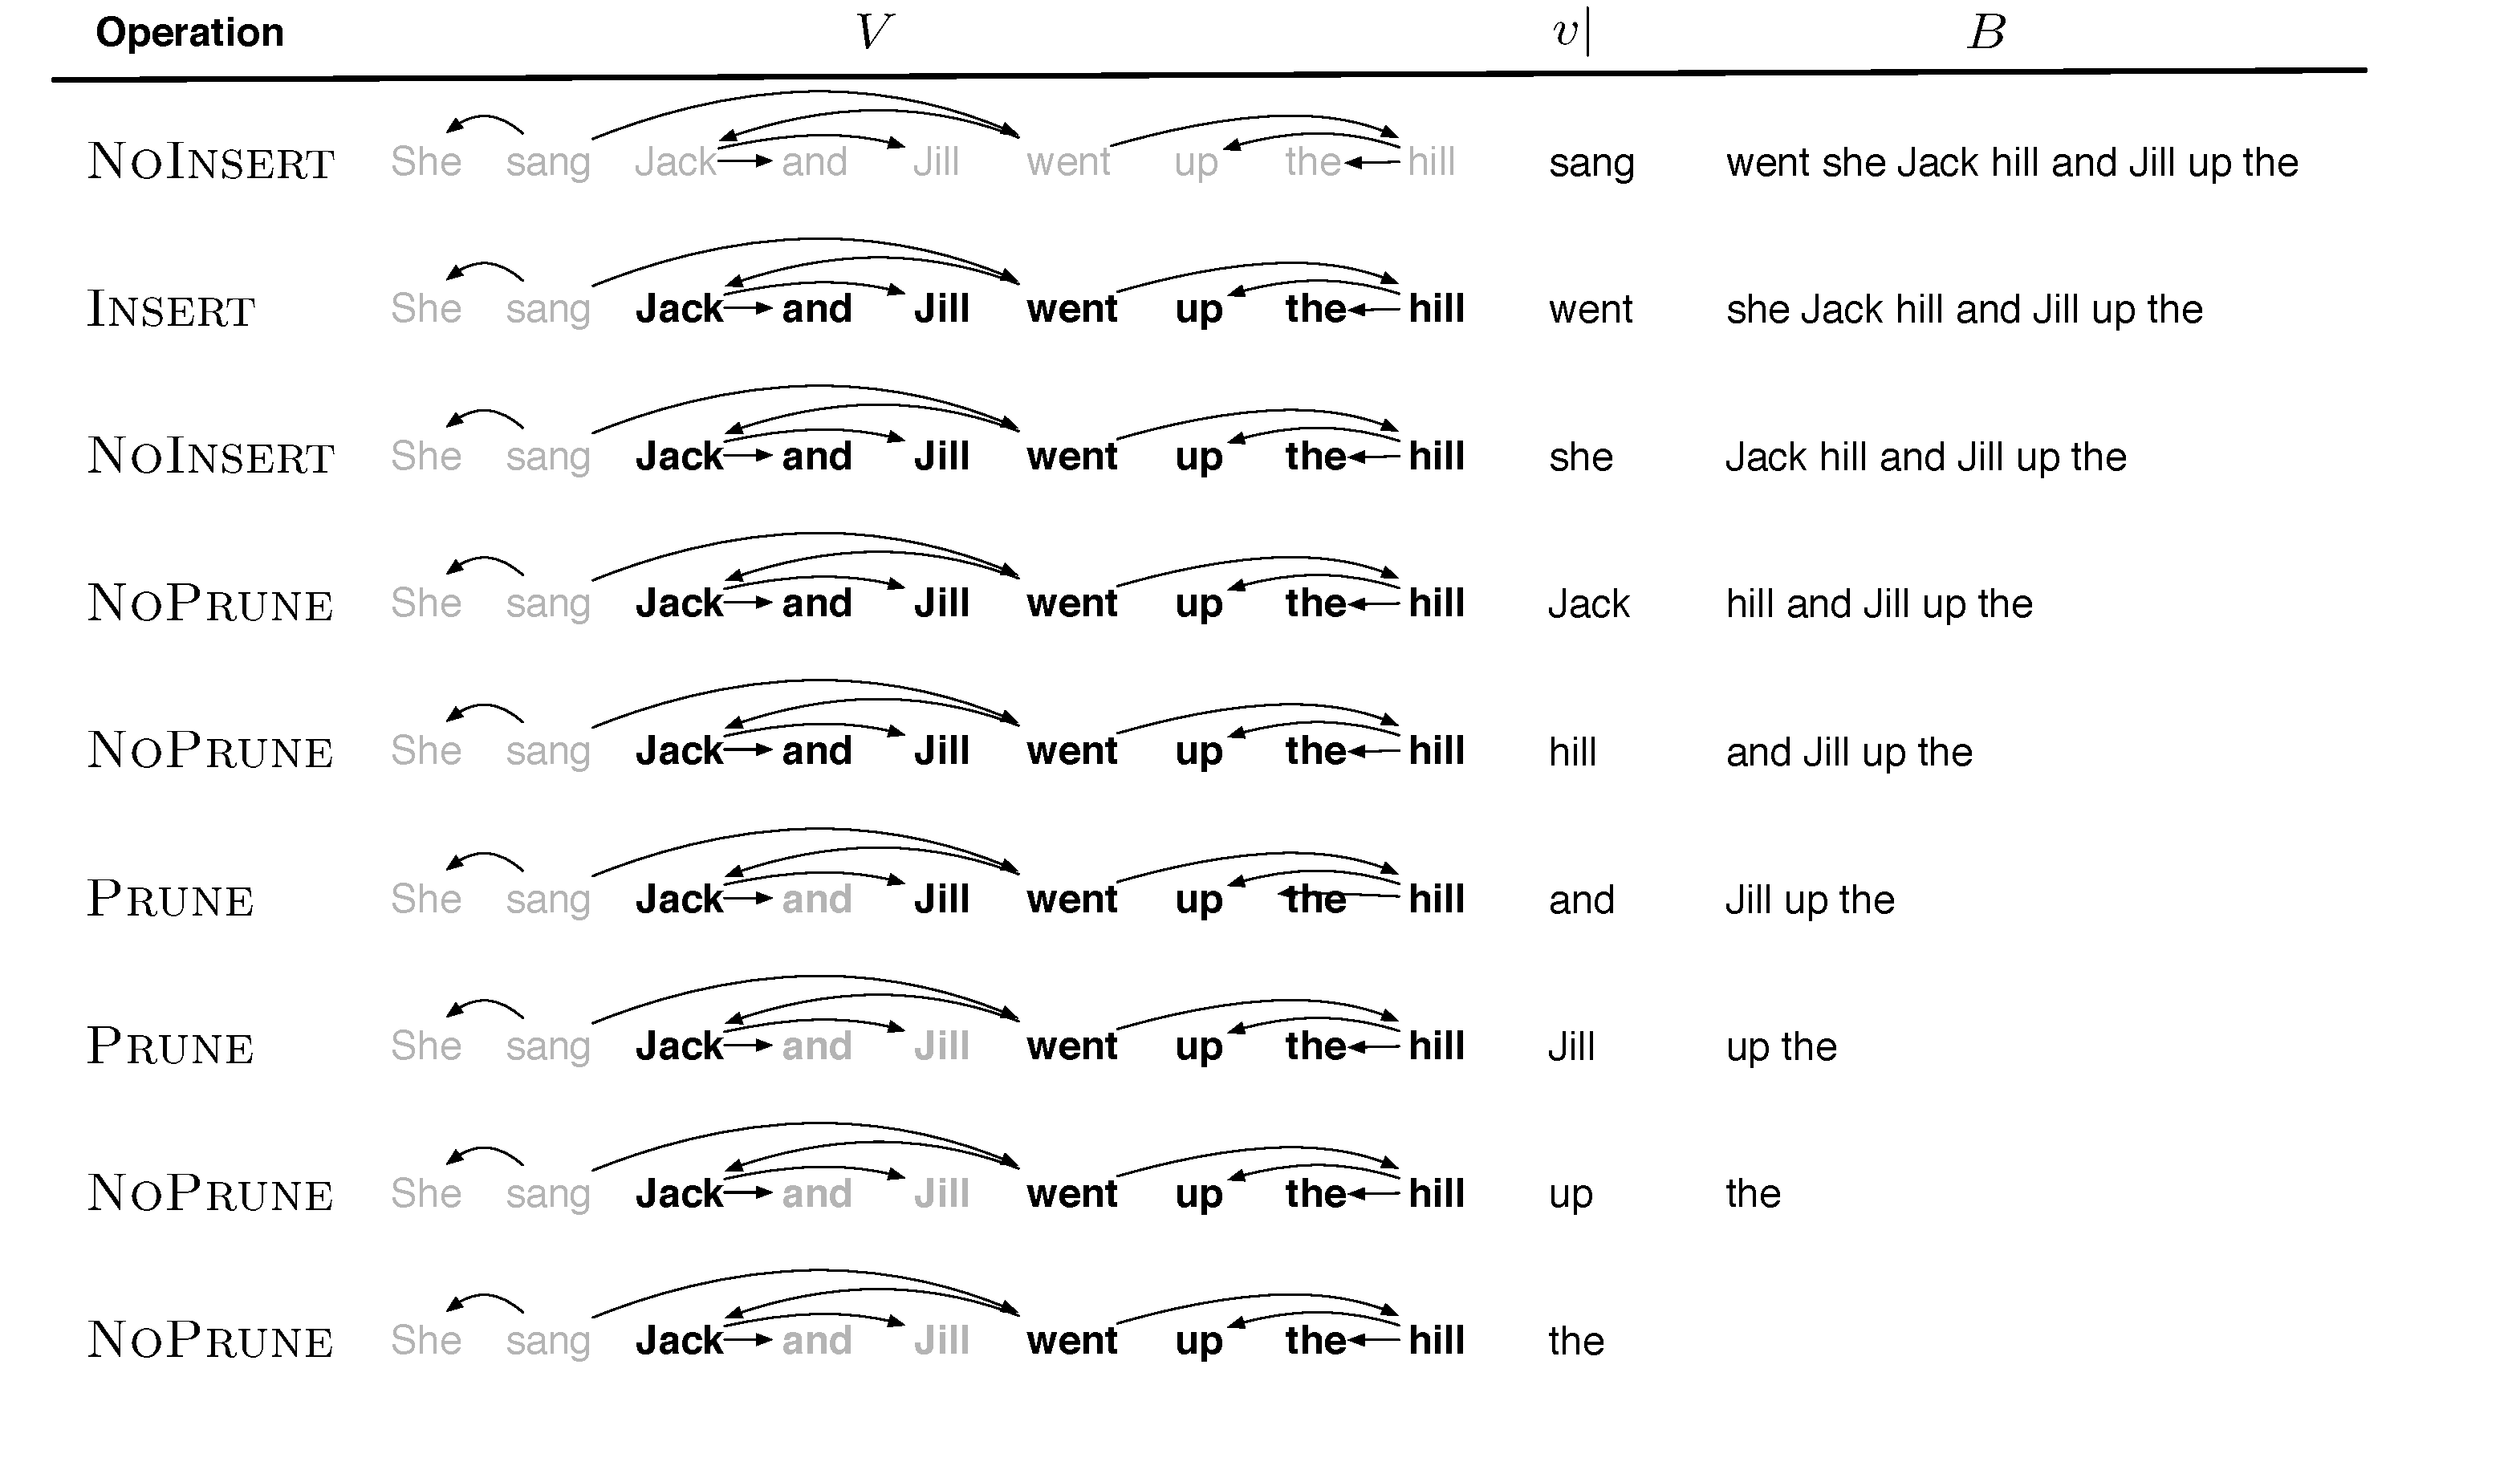
\includegraphics[width=.75\textwidth]{worked.pdf}
\caption{Nine operations of our transition-based compression return the compression: ``Jack went up the hill". At each timestep, the compression has state $(V, [v|B])$. In the diagram, the tokens in $V$ are shown in bold. At each timestep, the token $v$ at the head of the buffer $B$ is shown in the third column. Our compression system references the original, unchanging dependency parse of the sentence, $s$, shown in the diagram. The buffer is initialized breadth-first. Compression stops when the buffer is empty.}
\label{f:example}
\end{figure*}

\subsection{Reimplementation of \citet{filippova2013overcoming}: additional details}

In this work, we reimplement the method of \citet{filippova2013overcoming}, who in turn implement a method partially described in \citet{filippova2008dependency}.  There are inevitable discrepancies between our implementation and the ILP methods described in these two prior papers.  

Some discrepancies arise from differences in syntactic formalisms. To begin, prior work uses a tree transformation method which is no longer strictly compatible with UD. For instance, the tree transformation from prior work assumes PPs are headed by prepositions, which is not true in UD \cite{Schuster2016EnhancedEU}. In implementing the ILP, we use the enhanced dependencies representation from CoreNLP \cite{Schuster2016EnhancedEU}. The augmented modifiers and augmented conjuncts in this representation create parses that are very similar to the transformed trees described in prior work. \citet{filippova2008dependency} also describe a syntactic constraint based on the \rdep{sc} relation, which is not included in UD. We therefore exclude this constraint.

Other possible discrepancies arise from differences in part-of-speech taggers. In particular, prior work modifies a dependency tree by adding an edge between the root note and all verbs in a sentence, as a preprocessing step. This ensures that subclauses can be removed from parse trees, and then merged together to create a compression from different clauses of a sentence. However, we found that replicating this transform literally (i.e. only adding edges from the original root to all ``verbs'') made it impossible for the ILP to recreate some of the gold compressions in the dataset. (We suspect that this is because our part-of-speech tagger and the original part-of-speech tagger employed in \citet{filippova2013overcoming} sometimes return different part-of-speech tags). Our tree transform therefore adds an edge between the root node and \textit{all} tokens in a sentence. With this change, it is always possible for the ILP to output the gold compression.

We use \citet{gurobi} (v7) to solve the liner program. \citet{filippova2008dependency} report using LPsolve.\footnote{\url{http://
sourceforge.net/projects/lpsolve}}  We found that Gurobi sometimes segfaults nondeterminsitically during training. We implement checkpoints which save and restore the state of computation, allowing us to resume training when such errors occur.  We assess convergence by examining the validation F1 score on the contrained task after each pass through the training data. The F1 score increases for each of eight passes through the training data, and then decreases by $10^{-3}$). We thus terminate training. 

Lastly, in Table 1 of their original paper, \citet{filippova2013overcoming} provide an overview of the syntactic, structural, semantic and lexical features in their model. We implement every feature explicitly described in their work, except where otherwise noted (e.g. syntactic feature not compatible with UD). However, additional features implemented in their model (but not not described in their overview) almost certainly affect performance. 


\subsection{Implementation of SLOR: additional details}

We use the SLOR function to measure the readability of the shortened sentences produced by each compression system. Following \cite{lau2015unsupervised}, we define the function as 

\begin{equation}
\text{SLOR}=\frac{\text{log}P_m(\xi) - \text{log}P_u(\xi)}{|\xi|}
\end{equation}

where $\xi$ is a sequence of words, $P_u(\xi)$ is the unigram probability of this sequence of words and $P_m(\xi)$ is the probability of the sequence, assigned by a language model.  $|\xi|$ is the length (in tokens) of the sentence.

We use a 3-gram language model trained on the \citet{filippova2013overcoming} corpus. We implement with KenLM \cite{Heafield-kenlm}.

\subsection{Subtree and compression brackets: additional details}\label{s:subtree}

Our markup input to our LSTM, $\bm{x_j}$, includes \textbf{subtree brackets} with a complex structure, used to represent the start and end of the tokens which will be pruned or inserted by an operation $o_j \in \{ \textsc{Prune},\textsc{Insert}\}$. The start and end tags are each formed by concatenating two symbols: (1) a symbol $o_j$ indicating the type of the operation proposal (i.e. prune or insert) and (2) a symbol $d$ indicating the dependency type governing $T(v)$, such as \texttt{dobj}. 

Additionally, the markup includes \textbf{compression brackets} which show the extent of the current compression (if the operation is \textsc{Prune}) or the extent of the compression which would result if the operation were to be accepted (if the operation is \textsc{Insert}). Concretely, these brackets show the extent of \textsc{Max}($V_{j+1}, V_{j}$) within $s$ where, \textsc{Max} selects the largest set by cardinality and where $V_{j+1}$ is all tokens which would be in $V$ at step $j+1$, if the system were to execute operation $o$ at timestep $j$. If $o_j=\textsc{Prune}$ then $V_{j+1}$ will be smaller than $V$ and the bracket symbols will show the extent of the current $V_j$. If $o_j=\textsc{Insert}$, then $V_{j+1}$ will be larger than $V_j$ and the compression brackets will show the extent of the compression which would result if the tokens were to be inserted at timestep $j$. 

\begin{table}[htb!]
\begin{tabular}{@{}ll@{}}
\toprule
Batch size         & 135                      \\ 
Hidden size        & 907                        \\
Embeddings dim.    & 300                      \\
Total fully-connected layers & 2                        \\
Fully-connected layers, hidden sizes & $(92, 2)$ \\
Fully-connected layers, dropout & $(0.3093, 0.4078)$ \\
Fully-connected layers, activations        & Relu, Linear             \\
Learning rate      & $4.593 * 10^{-4}$   \\
Weight decay       & $2.421 * 10^{-8}$   \\ \bottomrule
\end{tabular}
\caption{The hyperparameters for our model. We optimize hyperparameters via random search \cite{Bergstra2012RandomSF}. The learning rate and weight decay parameter each clearly affect validation accuracy. The importance of other parameters is less clear. } 
\end{table}

\subsection{Neural net training: additional details}

We note several additional details about our neural network training procedure.

\begin{itemize}
\item{We train on 8 million tuples. The cardinality of the training set was bounded by available hardware resources, not by the total number of oracle tuples which can be generated with the \citet{filippova2013overcoming} dataset.}
\item{We weight each training instance $(\bm{x}, y_i)$ using $\frac{T_o}{2 * T_{o,i}}$, the default class weighting scheme in Scikit-learn \cite{Pedregosa:2011:SML:1953048.2078195}. $T_o$ is the total number of training examples of accepted and rejected instances of the operation proposal $o$ (e.g. $T_o$ = total number of \textsc{Prune} examples + total number of \textsc{NoPrune} examples). $T_{o,i}$ is the total number of training operations labeled $y_i$ for operations of proposal type $o$ (e.g. $T_{i,o}$ = the total \textsc{NoPrune} operations, if $y_i=0$ and instance is of type \textsc{Prune}). The 2 in the numerator denotes the total number of classes. Alternative weighting methods are left for future work.}
\item{We also experimented with ELMo vectors \cite{Peters:2018}, but found that we were able to achieve similar validation accuracies with much smaller embeddings, and so did not pursue further work with ELMo. It is possible that ELMo-like vectors could be used to increase performance in the future.}
\end{itemize}
